% document setup
\documentclass[12pt,a4paper]{article}
\usepackage[utf8]{inputenc}
\usepackage[ngerman]{babel}

% maths
\usepackage{amsfonts}
\usepackage{amssymb}
\usepackage{amsmath}

% utility
\usepackage{xcolor}
\usepackage{float}
\usepackage[colorlinks=false,linkbordercolor=red,urlbordercolor=red]{hyperref}
\usepackage[shortlabels]{enumitem}
\usepackage{tikz}

% useful commands
\newcommand{\qed}{\null\nobreak\hfill\square}

% title, author etc.
\title{Analysis I, Blatt 1}
\author{
    Gruppe 11\\
    Lorenz Bung (Matr.-Nr. 5113060)\\
    \href{mailto:lorenz.bung@students.uni-freiburg.de}{\texttt{lorenz.bung@students.uni-freiburg.de}}\\
    Charlotte Rothhaar (Matr.-Nr. 4315016)\\
    \href{mailto:charlotte.rothhaar97@gmail.com}{\texttt{charlotte.rothhaar97@gmail.com}}
}
\date{\today}

% begin document
\begin{document}

\maketitle


\section*{Aufgabe 1}

\begin{enumerate}[(i)]
    \item $f^{-1}(C \cap D) = \{x \in A | f(x) \in C \cap D\} = \{x \in A | f(x) \in C \wedge f(x) \in D\} \overset{C,D \subseteq B, f(x) \in B}{=} \{x \in A | f(x) \in C\} \cap \{x \in A | f(x) \in D\} = f^{-1}(C) \cap f^{-1}(D).$
    \item Sei $E := (- \infty; 0]$ und $F := [0; \infty)$, sowie $f: x \mapsto x^2$. Dann ist $$f(E \cap F) = f(\{0\}) = \{0\}$$ aber $$f(E) \cap f(F) = f((- \infty; 0]) \cap f([0; \infty)) = [0; \infty).$$
    \begin{minipage}[h]{\textwidth}
        \centering
        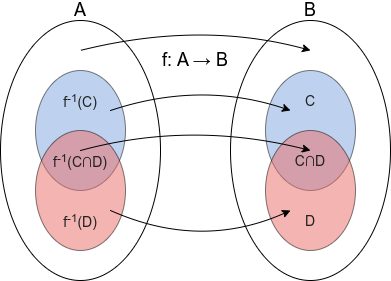
\includegraphics[width=0.5\textwidth]{Diagramm.png}
    \end{minipage}
    \item \begin{enumerate}[(a)]
        \item Angenommen, $f$ ist injektiv und es gibt Teilmengen $E, F \subset B$ mit $f(E \cap F) \subsetneq f(E) \cap f(F)$.
        Dann gäbe es ein $y \in f(E) \cap f(F)$ mit $y \notin f(E \cap F)$.
        Somit: $\exists x_1 \in E, x_2 \in F: f(x_1) = f(x_2) = y$.
        Nach Injektivität darf jedoch jedes Element aus dem Bild von $f$ nur ein Urbild haben, weswegen $x_1 = x_2$.
        Widerspruch! $\Rightarrow$ Gleichheit.
        \item
    \end{enumerate}
\end{enumerate}


\section*{Aufgabe 2}

\begin{enumerate}[(i)]
    \item \begin{itemize}
        \item \textit{injektiv}: Ja, da keine zwei natürlichen Zahlen denselben Nachfolger haben (folgt direkt aus dem 4. Peanoaxiom). Daher muss $\nu$ injektiv sein.
        \item \textit{surjektiv}: Nein. Nach dem 1. Peanoaxiom ist $0 \in \mathbb{N}.$ Das 3. Axiom besagt jedoch, dass $\nexists x \in \mathbb{N} : \nu(x) = 0.$ Daher kann $\nu$ nicht surjektiv sein.
        \item \textit{bijektiv}: $\nu$ kann nicht bijektiv sein, da die Surjektivität bereits nicht gegeben ist.
    \end{itemize}
    \item \begin{enumerate}[(a)]
        \item Seien $a, b \in X, a \neq b$.
        Dann ist aufgrund der Injektivität von $f$ $f(a) \neq f(b)$.
        Da auch $g$ injektiv ist, folgt $g(f(a)) \neq g(f(b)) \Leftrightarrow (g \circ f)(a) \neq (g \circ f)(b)$.
        Die Aussage ist also wahr, weil auch $g \circ f$ injektiv ist.
        \item Falsch. Gegenbeispiel: Sei $f: \mathbb{N} \rightarrow \mathbb{N}$ mit $f: x \mapsto x+1$ und $g: \mathbb{N} \rightarrow \{1\}$ mit $g: x \mapsto 1.$ $f$ ist injektiv, da die Nachfolgerfunktion schon injektiv ist. $g$ ist surjektiv, da auf jedes Element aus $\{1\}$ (nämlich nur die $1$ selbst) abgebildet wird (z.B. ist $g(1) = 1$). $g \circ f$ kann jedoch nicht injektiv sein, da $(g \circ f) (1) = g(f(1)) = g(2) = 1 = g(3) = g(f(2)) = (g \circ f) (2)$.
        \item Sei $a \in Z$.
        Aufgrund der Surjektivität von $g$ gilt: $\exists c \in Y: g(c) = a.$
        Da auch $f$ surjektiv ist, folgt $\exists b \in X: f(b) = c.$
        Somit ist $(g \circ f)(b) = g(f(b)) = g(c) = a$ und damit ist auch $g \circ f$ surjektiv.
        \item
    \end{enumerate}
\end{enumerate}


\section*{Aufgabe 3}

\begin{enumerate}[(i)]
    \item \begin{enumerate}[(a)]
        \item Zeige zunächst $A(n) \Rightarrow A(n+1)$:\\
        Induktionsbehauptung (IB): $\sum\limits_{k=0}^n k * k! = (n + 1)! + 1.$\\
        Induktionsschritt (IS): $\sum\limits_{k=0}^{n+1} k * k! = \sum\limits_{k=0}^n k * k! + (n + 1) * (n + 1)! \overset{\text{(IB)}}{=} (n + 1)! + 1 + (n + 1) * (n + 1)! = (n + 1)! * (1 + (n + 1)) + 1 = (n + 1)! * (n + 2) + 1 = (n+2)! + 1.$\\\\
        Zeige nun $B(n) \Rightarrow B(n+1)$:\\
        Induktionsbehauptung (IB): $\sum\limits_{k=0}^n k*k! = (n+1)!-1.$\\
        Induktionsschritt (IS): $\sum\limits_{k=0}^{n+1} k*k! = (n+1)!-1 = \sum\limits_{k=0}^n k*k! + (n+1)*(n+1)! \overset{\text{(IB)}}{=} (n+1)!-1+(n+1)*(n+1)! = (n+1)!*(1+n+1)-1 = (n+1)!*(n+2)-1 = (n+2)!-1.$
        \item Zum Beweis der Aussagen für alle $n \in \mathbb{N}$ fehlt der jeweilige Induktionsanfang. Es wurde zwar die Implikation gezeigt, jedoch nicht, dass die Aussage überhaupt für das erste Element gilt.\\
        Um zu zeigen, dass $B(n)$ für alle $n \in \mathbb{N}$ gilt, genügt nun der Induktionsanfang ($n=0$): $\sum\limits_{k=0}^0 k*k! = 0*0! = 0 = 1!-1 = (0+1)!-1.$
    \end{enumerate}

    \item \begin{itemize}
        \item \textit{Fall 1:} $n$ ist durch $m$ teilbar.\\
        Dann ist $q = \frac{n}{m} \Leftrightarrow n = q * m$.
        Setze $r := 0$: $n = q * m + 0 = q * m + r.$
        \item \textit{Fall 2:} $n$ ist nicht durch $m$ teilbar.\\
        Dann existiert eine Zahl $x \in \mathbb{N}$ mit $x > n$, die durch $m$ teilbar ist, also $\frac{x}{m} = q \Leftrightarrow x = q * m.$\\
        Da $x > n$ lässt sich $x$ schreiben als $x = n + (n - n)$ und ferner $n + (x - n) = q * m.$\\
        Wähle nun $r := -(x-n).$ Dann ist $n + (x - n) = n - r = q * m \Leftrightarrow n = q * m + r.$\\
        $\qed$
    \end{itemize}
\end{enumerate}


\section*{Aufgabe 4}

\begin{itemize}
    \item \textit{Fall 1:} \begin{equation}
    \label{a4:eq1}
        a \geq 0 \wedge b \geq 0.
    \end{equation}
    Dann ist $|a| = a$ und $|b| = b$, und somit $|a| + |b| = a + b \geq 0.$
    Aus (\ref{a4:eq1}) folgt $a + b \geq 0$ und daher auch $|a+b| \geq 0.$
    Es bleibt also zu zeigen, dass
    \[
    a + b \leq a + b + |a-b| \Leftrightarrow 0 \leq |a-b|.
    \]
    Ist $a \geq b$, dann ist $0 \leq a - b$ und somit $|a-b| = a-b.$ Dann gilt jedoch bereits $0 \leq |a-b| = a-b.$
    Ist $a < b$, so ist $a-b < 0$ und damit $|a-b| = -(a-b).$ Dann ist jedoch $|a-b| = -(a-b) > 0$.
    \item \textit{Fall 2:} \begin{equation}
        \label{a4:eq2}
        a < 0 \wedge b < 0.
    \end{equation}
    Dann ist $|a| = -a$ und $|b| = -b$, und somit $|a| + |b| = -a-b.$
    Aus (\ref{a4:eq2}) folgt $a + b < 0$ und somit $|a + b| = - (a + b) = -a-b.$
    Es bleibt also zu zeigen, dass
    \[
    -a-b \leq -a-b + |a-b| \Leftrightarrow 0 \leq |a-b|.
    \]
    Ist $a < b$, dann ist $a-b < 0$ und damit $|a-b| = -(a-b) > 0$.
    Ist $a \geq b$, dann ist $a-b \geq 0$ und $|a-b| = a-b \geq 0$.
    \item \textit{Fall 3:} \begin{equation}
        \label{a4:eq3}
        a \geq 0 \wedge b < 0.
    \end{equation}
    Dann ist $|a| = a$ und $|b| = -b$, sowie $b < a$. Weiterhin ist $|a| + |b| = a-b$.\\
    Aus (\ref{a4:eq3}) folgt $-b > 0$ und damit $a-b > 0$. Daher ist $|a-b| = a-b$.
    Es bleibt also zu zeigen, dass
    \[
    a-b \leq |a+b| + a-b \Leftrightarrow 0 \leq |a+b|.
    \]
    Ist $a + b \geq 0$, dann ist $|a+b| = a+b \geq 0$.
    Ist $a+b < 0$, so ist $|a+b| = - (a + b) > 0$.
    \item \textit{Fall 4:} \begin{equation}
    \label{a4:eq4}
        a < 0 \wedge b \geq 0.
    \end{equation}
    Dann ist $|a| = -a$ und $|b| = b$, sowie $|a| + |b| = -a+b$.
    Aus (\ref{a4:eq4}) folgt $-b \leq 0$.
    Damit ist $a-b < 0$ und $|a-b| = -(a-b) = -a+b$.
    Es bleibt also zu zeigen, dass
    \[
    -a+b \leq |a+b|-a+b \Leftrightarrow 0 \leq |a+b|.
    \]
    Ist $a+b \geq 0$, dann ist $|a+b| = a+b \geq 0$.
    Ist $a+b < 0$, so ist $|a+b| = -(a+b) > 0$.
\end{itemize}
$\qed$

Es gilt Gleichheit, wenn $a \leq b \wedge a \geq b \Leftrightarrow a = b$.


% end document
\end{document}